%
\begin{tikzpicture}[remember picture, overlay, shift=(current page.center)]
  \node at (0, -0.25) {%
    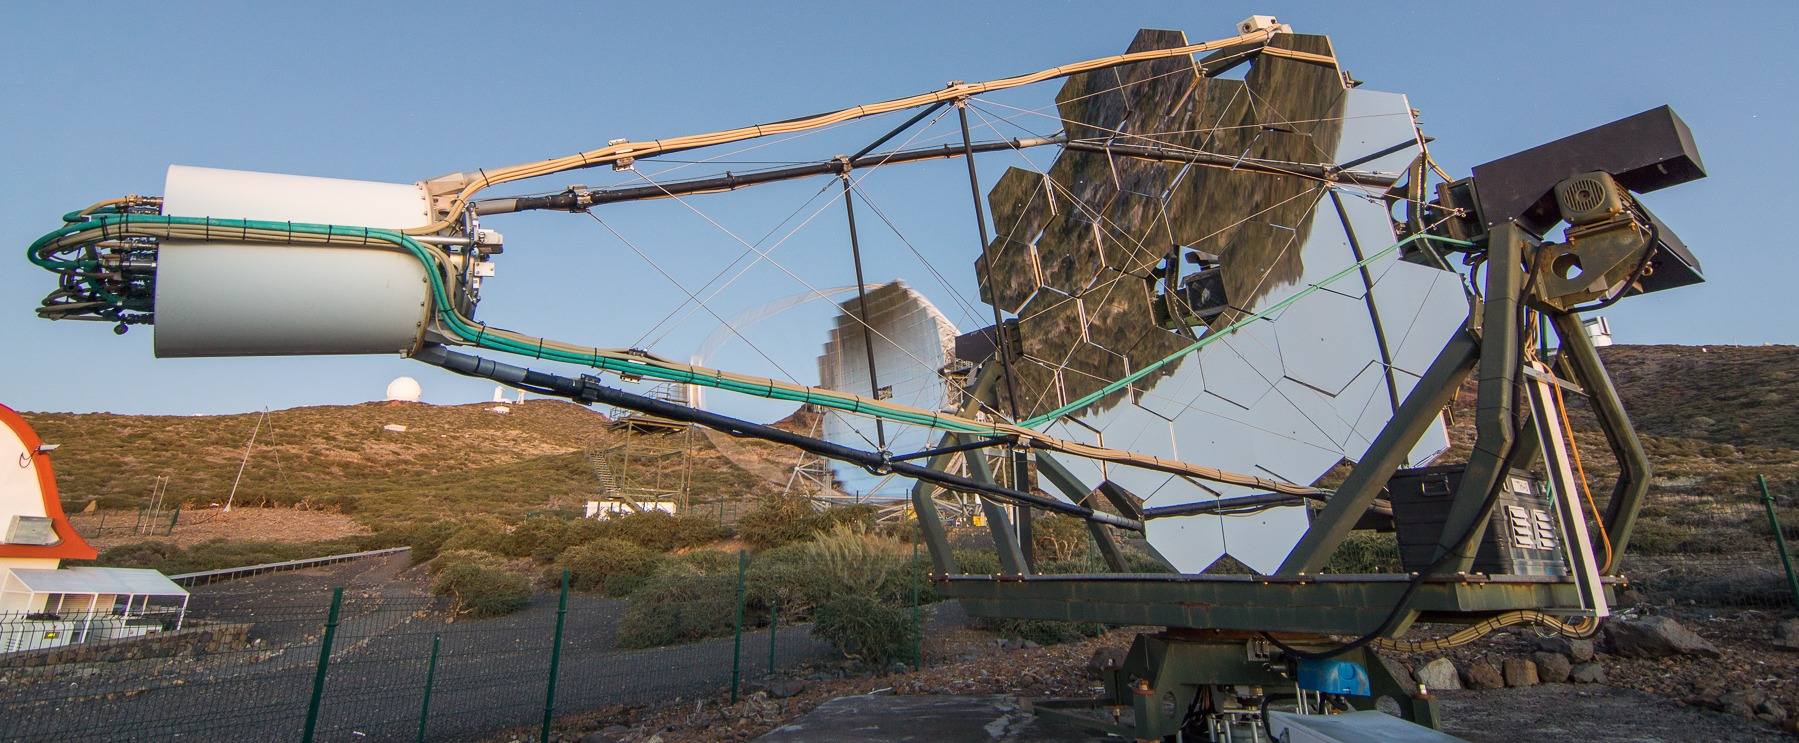
\includegraphics[width=\linewidth, height=0.95\textheight, keepaspectratio]{images/fact.jpg}%
  };
\end{tikzpicture}%
%
\only<2>{%
  \begin{tikzpicture}[remember picture, overlay, shift=(current page.center)]
    \node (camera) at (-5.25, 0.5) {%
      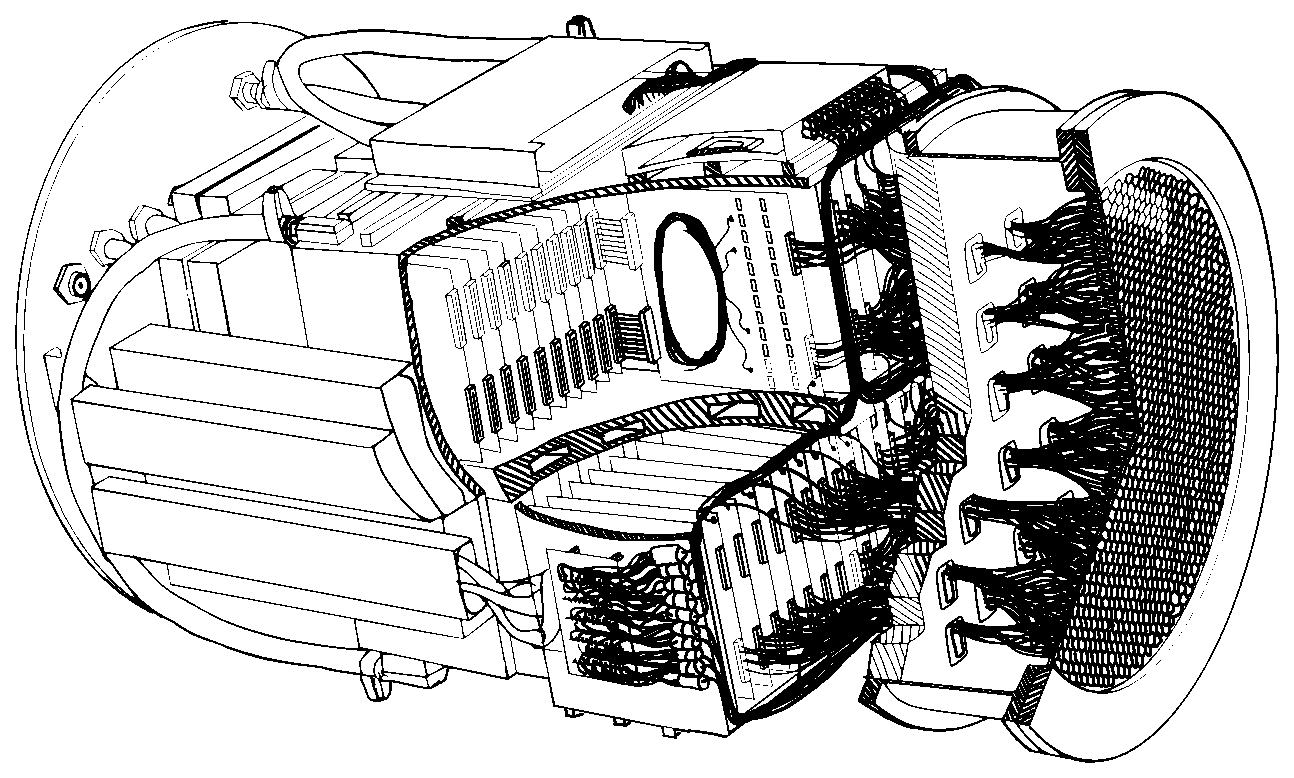
\includegraphics[width=4cm]{images/image_sensor_filled.pdf}%
    };
    \node[text=white, rotate=-4] at (camera.north) {[S.\,A.\,Mueller]};
    \node[anchor=north west, text width=7.5cm, fill=white, opacity=0.9, text opacity=1.0] at (camera.340) {
      \begin{itemize}
        \item 1440 SiPM Pixel à 3600 G-APD Zellen
        \item Robust, auch bei Mondlicht
        \item 2 GSample/s Auslese
        \item Trigger: 60–80 Ereignisse / Sekunde
        \item 300 Messwerte pro Pixel pro Ereignis
      \end{itemize}
      \vspace{0.5\baselineskip}
    };
  \end{tikzpicture}%
}%
%
\only<3>{%
  \begin{tikzpicture}[remember picture, overlay, shift=(current page.center)]

    \coordinate (center) at (2.5, 0.4);
    \draw[tugreen, line width=3pt] (center) ellipse[x radius=2, y radius=2.4, rotate=18];
    \draw[tugreen, line width=3pt, -{Triangle}] (center) -- ++(18:2cm);
    \draw[tugreen, line width=3pt, -{Triangle}] (center) -- ++(18:-2cm);


    \node[anchor=north, text width=2cm, rotate=18, yshift=-0.05cm, fill=white, opacity=0.9, text opacity=1.0] at (center) {%
      \setlength{\abovedisplayskip}{0pt}%
      \begin{align*}%
        \oslash &≈ \SI{3.6}{\meter} \\
        A &= \SI{9.5}{\square\meter}
      \end{align*}%
    };
    \draw[tugreen, line width=3pt, -{Triangle}] (center) -- (-3.5, 0.5) node[
      midway, above, fill=white, opacity=0.9, text opacity=1, text=darkgray
    ] {$f = \SI{4.9}{\meter}$};

    \node[fill=white, opacity=0.9, text opacity=1, text=darkgray, anchor=east, circle] at (-3.5, 0.5) {\SI{4.5}{\degree}-Sichtfeld};


  \end{tikzpicture}%
}%
%
